%==============================================================================
\chapter{In silico mapping sarcomere pharmacological modulations to whole-organ function and back again: the omecamtiv mecarbil case study}\label{cha:chapter5}
%==============================================================================
%
%
%
\begin{remark}{Outline}
    In this chapter, we use the personalised SHAM rat heart contraction model as a reference model of a healthy rat to show that it is possible to quantitatively map pharmacological interventions at the sarcomere level through to whole-organ function. Moreover, we show that we can infer cell-level compound effects from whole-organ observations, making the inverse mapping possible. We apply this framework to an example drug, namely to omecamtiv mecarbil, which has been proposed as a possible treatment of heart failure with reduced ejection fraction.
\end{remark}


%
%
%
\section{Motivation}\label{sec:ch5motivation}
\todo{this is Abstract, Introduction copy-pasted from the paper: adapt it to thesis}

\noindent
Omecamtiv mecarbil (OM) is a cardiac myosin activator developed as a treatment of heart failure. OM acts on cross-bridge formation without disrupting intracellular calcium homeostasis. OM effects are extensively characterised both \textit{in vitro} and \textit{in vivo} yet how these mechanistically translate from the sarcomere to whole-heart function is not fully understood. We employed a $3$D biventricular contraction model of a healthy rat heart that was fitted to anatomic, structural, and hemodynamic and volumetric functional data. The model incorporates pre-load, after-load, fibre orientation, passive material properties, anatomy, calcium transients, and thin and thick filament dynamics. We identified $4$ sarcomere model parameters that reflect cross-bridge behavior. Gaussian process emulators (GPEs) were trained to map these parameters to pressure- and volume-based indexes of left ventricular (LV) function. We constrained the $4$-parameter space using preclinical OM data, either ($1$) \textit{in vivo} whole-heart hemodynamics data (using the Bayesian history matching technique), or ($2$) \textit{in vitro} F-pCa measurements. The OM-compatible sarcomere parameter space from case ($1$) was used to directly calculate F-pCa curves, while the one resulting from case ($2$) was mapped to the LV indexes using the trained GPEs. We found that our mapping from LV features to F-pCa and vice versa was in agreement with experimental data. In addition, our simulations supported the latest evidence that OM indirectly alters thin filament calcium sensitivity. Our work demonstrates how quantitative mapping from cellular to whole-organ level can be used to improve our understanding of drug action mechanisms.

\vspace{0.2cm}
Heart failure (HF) is a leading cause of hospitalisation worldwide, with more than one million admissions annually in the US and Europe~\cite{Benjamin:2018}. However, the treatment options are limited and, therefore, new pharmacotherapies are continuously sought. HF pathways can involve impaired cellular function and propagate up to the whole-organ dysfunction. Multi-scale contraction modelling represents a useful tool for understanding the underlying mechanisms and possibly identifying targets in these pathways.

Building on a previously developed multi-scale rat bi-ventricle mechanics modelling framework~\cite{Longobardi:2020}, we can investigate drug mechanisms of action and better understand the mechanistic processes linking cellular and whole-heart contraction. For this case study, we chose omecamtiv mecarbil (OM), a novel drug currently in Phase $3$ clinical trial~\cite{Teerlink:2021} for treating HF. OM is a selective allosteric cardiac myosin modulator. It increases the rate of cross-bridge cycling by accelerating phosphate release~\cite{Malik:2011}, without disrupting intracellular calcium dynamics~\cite{Horvath:2017}. Recently, OM was shown to enhance the duty ratio, resulting in increased calcium sensitivity and slowed force development~\cite{Swenson:2017, Kampourakis:2018}.

This paper outlines our methodology of incorporating OM into our model, that consists of calibrating the cellular model using \textit{in vitro} data from skinned cellular and trabecular preparations in OM-containing solutions~\cite{Nagy:2015,Kampourakis:2018,Kieu:2019}, and validating the biventricular multi-scale contraction model using pressure-volume measurements from \textit{in vivo} whole-heart studies in healthy animals with OM~\cite{Bakkehaug:2015}. Our simulation results are consistent with the available experimental data on OM and support the hypothesis (e.g.~\cite{Swenson:2017}) that OM affects the thin filament.

%
%
%
\section{Preclinical data}\label{sec:ch5preclinicaldata}

%
%
%
\subsection{Cell-level measurements}\label{sec:ch5celllevelmeasurements}
\textit{In vitro} measurements of the OM effects on the sarcomere in healthy rats were taken from literature experimental studies performed on skinned myocytes' preparations. OM effects were given in terms of alterations of the $\pCaf$ and $h$ features of the F-pCa curve (introduced in Section~\ref{sec:ch2theforcecalciumrelationship}, equation~\eqref{eq:FpCa}). To map these effects from skinned to intact/\textit{in vivo} results we used percentages of F-pCa featueres' change from the control muscle to the OM-containing solution-exposed muscle. These values are summarised in Table~\ref{tab:pshiftpslope}.

\begin{table}[!ht]
    \myfloatalign
    \begin{tabularx}{\textwidth}{lXX}
    \toprule
    \tableheadline{Fraction of change} & \tableheadline{Exp. variability} & \tableheadline{Reference}  \\
    \midrule
    $P_{\textrm{shift}}$ (for $\pCaf$) & $[0.0085,\,0.0833]$ & \cite{Nagy:2015, Kampourakis:2018, Kieu:2019} \\
    $P_{\textrm{slope}}$ (for $h$) & $[-0.7282,\,-0.2470]$ & \cite{Nagy:2015, Kampourakis:2018, Kieu:2019} \\
    \bottomrule
    \end{tabularx}
    \caption{F-pCa fractions of change experimental variability in OM-containing solution-exposed healthy rat skinned muscles. Values are given as ranges of minimum and maximum fractions of change from control experimental mean values.}
    \label{tab:pshiftpslope}
\end{table}



%
%
%
\subsection{Whole-organ measurements}\label{sec:ch5wholeorganlevelmeasurements}
We did not have \textit{in vivo} measurements of the OM effects on the whole-organ function in healthy rats, so qualitative observations from a healthy pig study were used~\cite{Bakkehaug:2015}. Again, we used percentage changes in LV features from baseline values after OM administration. In particular, we focused on the features whose change from control was reported to be statistically significant. These values are summarised in Table~\ref{tab:pigdata}.

\begin{table}[!ht]
    \myfloatalign
    \begin{tabularx}{\textwidth}{lXX}
        \toprule
        \tableheadline{LV feature} & \tableheadline{Exp. variability ($\SI{}{\percent}$)} & \tableheadline{Reference} \\
        \midrule
        $\textrm{EDV}^*$ & $87.14 \pm 17.14$ & \cite{Bakkehaug:2015} \\
        $\textrm{ESV}^*$ & $76.92 \pm 20.51$ & \cite{Bakkehaug:2015} \\
        $\textrm{SV}$ & $100.00 \pm 25.81$ & \cite{Bakkehaug:2015} \\
        $\textrm{EF}$ & $115.91 \pm 18.18$ & \cite{Bakkehaug:2015} \\
        $\textrm{ET}^*$ & $116.16 \pm 9.61$ & \cite{Bakkehaug:2015} \\
        $\textrm{Tdiast}^*$ & $88.24 \pm 16.97$ & \cite{Bakkehaug:2015} \\
        $\textrm{maxdP}^*$ & $121.66 \pm 35.53$ & \cite{Bakkehaug:2015} \\
        $\textrm{mindP}$ & $108.96 \pm 31.01$ & \cite{Bakkehaug:2015} \\
        \bottomrule
    \end{tabularx}
    \caption{Left ventricular features' experimental variability in healthy pigs after OM administration. Values are given as mean$\pm$std percentage change from control experimental mean values. Asterisked $(\cdot)^*$ features' changes were reported to be statistically significant.}
    \label{tab:pigdata}
\end{table}


%
%
%
\section{Methods}\label{sec:ch5methods}


%
%
%
\subsection{Rat heart contraction model}\label{sec:ch5ratheartcontractionmodel}
To quantitatively link sarcomere properties to whole-organ function, we used the personalised SHAM rat heart contraction model derived in Section~\ref{sec:ch4fittedmodels}. Again, this model (or simulator) can be seen as a multi-scale map from input parameters to output features.

\vspace{0.2cm}
With the simulator input, we aimed at modelling the OM effect at the sarcomere level.
As OM increases the rate of cross-bridge formation~\cite{Malik:2011}, we considered parameters that are specifically responsible for cross-bridge dynamics in the Land et al.~\cite{Land:2012} cell contraction sub-model, namely $\kxb$, $\nxb$, $\trpnf$ and $\tref$. These parameters, introduced in Section~\ref{sec:ch2contractionmodel} and again reported in Table~\ref{tab:paramswithdefom}, constituted the simulator $4$-dimensional input.

\begin{table}[!ht]
    \myfloatalign
    \begin{tabularx}{\textwidth}{llX}
    \toprule
    \tableheadline{Parameter} & \tableheadline{Units}                   & \tableheadline{Definition} \\
    \midrule
    $\kxb$                    & $\SI{}{\per\milli\second}$              & cross-bridges cycling rate \\
    $\nxb$                    & $-$                                     & cross-bridge formation degree of cooperativity \\
    $\trpnf$                  & $-$                                     & fraction of $\Ca$-TnC bounds for half-maximal cross-bridges activation \\
    $\tref$                   & $\SI{}{\kilo\pascal}$                   & maximal reference tension \\
    \bottomrule
    \end{tabularx}
    \caption{Model parameters and their definitions.}
    \label{tab:paramswithdefom}
\end{table}

\vspace{0.2cm}
The simulator output aimed at describing the LV function using a set of scalar features. These were the same $12$ features used in the previous analysis (Table~\ref{tab:lvfeatures}) with the addition of other $2$ features (Table~\ref{tab:lvfeaturesom}), for a total of $14$ features.

\begin{table}[!ht]
    \myfloatalign
    \begin{tabularx}{\textwidth}{llX}
    \toprule
    \tableheadline{LV feature}                  & \tableheadline{Units}                         & \tableheadline{Definition} \\ \midrule
    $\textrm{SV}$                  & $\SI{}{\micro\liter}$                  & stroke volume \\
    $\textrm{ET/Tdiast}$                  & $-$                  & systolic ejection time over diastiolic filling time \\
    \bottomrule
    \end{tabularx}
    \caption{Additional LV features of interest.}
    \label{tab:lvfeaturesom}
\end{table}

\noindent
The obtained simulator map had thus the following form:
%
\begin{align}\label{eq:fsimulom}
    f_{simul}\colon\mathbb{R}^{4} &\to\underbrace{\mathbb{R}\times\cdots\times\mathbb{R}}_{14\,\text{times}} \\
    \mathbf{x} &\mapsto (y_1,\,\dots,\,y_{14}) \nonumber
\end{align}

\noindent
When running the simulator at a new parameter point, we fixed all the parameters not included in the set of simulator inputs to the personalised SHAM rat model baseline parameter values (Table~\ref{tab:shamabbestfitparamvalues}) when applicable, or to the Land et al.~\cite{Land:2012} model baseline values when otherwise.


%
%
%
\subsection{Input parameter space}\label{sec:ch5inputparameterspace}
The input parameter space $X\subset\mathbb{R}^{4}$ of the simulator map $f_{simul}$ introduced in equation~\eqref{eq:fsimulom} was defined as the hypercube obtained by the Cartesian product of $4$ one-dimensional parameter ranges. Each of these ranges was given as the combination of bounds inferred from the \textit{in vitro} F-pCa data presented in Section~\ref{sec:ch5celllevelmeasurements} (further details are provided in Section~\ref{sec:ch5inferringomeffectswholeorganfpca}) and a $\pm\SI{50}{\percent}$ ($\pm\SI{30}{\percent}$ for $\tref$) perturbation around the related parameter reference value. Adopted ranges are reported in Table~\ref{tab:omparamranges}.

\begin{table}[!ht]
    \myfloatalign
    \begin{tabularx}{\textwidth}{XXX}
        \toprule
        \tableheadline{Parameter} & \tableheadline{Units} & \tableheadline{Range} \\
        \midrule       
        $\kxb$   & $\SI{}{\per\milli\second}$ & $[0.0086,\,0.0258]$ \\
        $\nxb$   & $-$ & $[0.90,\,7.05]$ \\
        $\trpnf$ & $-$ & $[0.05,\,0.50]$ \\
        $\tref$  & $\SI{}{\kilo\pascal}$ & $[109.25,\,202.89]$ \\
        \bottomrule
    \end{tabularx}
    \caption{Parameters' ranges used for describing the healthy rat model $4$D input parameter space.}
    \label{tab:omparamranges}
\end{table}



%
%
%
\subsection{Training dataset, emulators and global sensitivity analysis}\label{sec:ch5trainingdatasetandemulators}
We sampled $4096$ points from a LHD over the input parameter space $X$ defined in Section~\ref{sec:ch5inputparameterspace}. The simulator was run at these points, and the successfully completed simulations were collected to form the training dataset ($1189$ points).

\vspace{0.2cm}
Univariate GPEs, defined as in Section~\ref{sec:ch3gaussianprocessemulation}, were used to predict each of the $14$ LV output features, and all the GPE model hyperparameters (both from the mean function and from the zero-mean GP) were jointly optimised during training by maximisation of the model log marginal likelihood (equation~\eqref{eq:logmarginallikelihood}). The accuracy and adequacy of being used as a surrogate model for each of the resulting $14$ trained GPEs were evaluated using the $R^2$-score regression metric and the $ISE_2$, as described in Section~\ref{sec:ch3regressionaccuracy}. GPEs' implementation and training were performed using GPErks emulation tool~\cite{GPErks:2021} based on GPyTorch Python library~\cite{Gardner:2019}.

\vspace{0.2cm}
To study the input parameters' impact on the output LV features' total variance we performed a GSA using the trained GPEs. Model outputs' sensitivity to model inputs was characterised by Sobol' first-order and total effects. These were estimated using \texttt{SALib} Python library~\cite{Herman:2017}. GPErks tool~\cite{GPErks:2021} was used to incorporate GPEs' full posterior distribution samples to account for emulators' uncertainty in Sobol' indices estimates, by following the second emulation-based approach of equations~\eqref{eq:emulpostsamplesgsa1}--\eqref{eq:emulpostsamplesgsa2}, presented in Section~\ref{sec:ch3emulatorbasedestimates}. Parameters whose Sobol' indices' distributions' expectation was below the threshold $0.01$ were determined to have negligible effects.




%
%
%
\subsection{Inferring OM effects on whole-organ function from in vitro F-pCa measurements}\label{sec:ch5inferringomeffectswholeorganfpca}
We wanted to investigate whether it is possible to validate OM mechanisms of action by using the built quantitative link between sarcomere properties and whole-organ function.

\vspace{0.2cm}
By recalling equations~\eqref{eq:ec50}--\eqref{eq:h}:
%
\begin{align}
    & \pCaf = -\log\left[\Caift\left(\frac{\koff}{\kon}\frac{\trpnf}{1-\trpnf}\right)^{1/\ntrpn}\right] \\
    & h = \nxb\ntrpn(1-\trpnf)
\end{align}

\noindent
we can notice that among the $4$ chosen input parameters (Section~\ref{sec:ch5ratheartcontractionmodel}) there are $2$ parameters, namely $\trpnf$ and $\nxb$, that can be used to tune both the $\pCaf$ and $h$ at the same time. Given a set of changes $(\Delta\pCaf,\,\Delta h)$ in these two features of the F-pCa curve, it is possible to scale the $2$ parameters' reference values such that the F-pCa curve undergoes a perturbation of exactely $(\Delta\pCaf,\,\Delta h)$. This can be accomplished by solving for the set of scaling coefficients $(\alpha,\,\beta)\in\mathbb{R}\times\mathbb{R}$ the following equations:
%
\begin{align}
    & \pCaf(\mathbf{p}_{\textrm{new}}) - \pCaf(\mathbf{p}) = \Delta\pCaf \label{eq:pcafeqalpha} \\
    & h(\mathbf{p}_{\textrm{new}}) - h(\mathbf{p}) = \Delta h \label{eq:heqbeta}
\end{align}

\vspace{0.2cm}\noindent
where $\pCaf(\cdot)$ and $h(\cdot)$ are now seen as functions of the reference $\mathbf{p}=(\trpnf,\,\nxb)$ and the new $\mathbf{p}_{\textrm{new}}=(\alpha\cdot\trpnf,\,\beta\cdot\nxb)$ parameter vectors.

\vspace{0.2cm}
The resulting $2$-dimensional space given by all the possible $\mathbf{p}_{\textrm{new}}$ vectors obtained by solving equations~\ref{eq:pcafeqalpha}--\ref{eq:heqbeta} for all the viable $(\Delta\pCaf,\,\Delta h)$ according to the experimentally observed variability for the F-pCa curve (Table~\ref{tab:pshiftpslope}) will constitute an OM-compatible sarcomere space encoded by the $\trpnf$ and $\nxb$ parameters. We obtained this space by first generating a LHD of $100,000$ points in the fractions of change $2$D experimental space (Table~\ref{tab:pshiftpslope}), and then projecting this into the corresponding $2$D sarcomere parameter space as described above.

\vspace{0.2cm}
We finally mapped this space, while keeping $\kxb$ and $\tref$ parameters for which we had no data fixed to their reference values, to EDV, ESV, ET/Tdiast and maxdP features using the corresponding GPEs, in order to see if these features were moving in the direction of change experimentally observed in the \textit{in vivo} pig hemodynamics after OM administration (Section~\ref{sec:ch5wholeorganlevelmeasurements}).


%
%
%
\subsection{Inferring OM effects on the sarcomere from in vivo whole-organ measurements}\label{sec:ch5inferringomeffectsfpcawholeorgan}
We wanted to understand what the experimental \textit{in vivo} pig data of altered LV function with OM administration could tell about the sarcomere parameter space of the model. To do this, we used a single iteration of HM technique. This was done as described in Section~\ref{sec:ch3historymatching}, using the maximum implausibility measure
(equation~\eqref{eq:maximplmeasure}) across multiple target features, with the model discrepancy term (and its corresponding variance) set to zero in equation~\eqref{eq:implmeasure}.

\vspace{0.2cm}
For the target features, we aimed at matching the experimental variability observed in the LV features that showed a significant change from baseline after OM administration (Table~\ref{tab:pigdata}), and at keeping all the other features constant by matching for those an experimental variability of $\SI{100}{\percent}\pm\SI{0}{\percent}$ (i.e. no change). We sampled $400,000$ $NROY$ points from a LHD in the input parameter space $X$ (derived in Section~\ref{sec:ch5inputparameterspace}). As the GPEs had very high accuracy and very low variance for the predictions (shown in the results Section~\ref{sec:modelemulatorsandoutputsensitivities}), the HM single iteration was performed with half the common value for the implausibility cutoff, i.e. $I_{\,\textrm{cutoff}}=1.5$. This allowed to cut most of the space while still retaining few $X_{NIMP}$ points, as we shell see in Section~\ref{sec:ch5inferringomeffectsfpcawholeorganresults}.

\vspace{0.2cm}
The obtained $X_{NIMP}$ space constituted an OM-compatible sarcomere space encoded by the $\kxb$, $\nxb$, $\trpnf$ and $\tref$ parameters. The points from this space were finally mapped using the Land et al.~\cite{Land:2012} model of cellular contraction to F-pCa curves, in order to see if the corresponding $\pCaf$ and $h$ features were moving in the direction of change experimentally observed in rats' skinned muscle preparations in OM-containing solutions (Section~\ref{sec:ch5celllevelmeasurements}).


%
%
%
\section{Results}\label{sec:ch5results}


%
%
%
\subsection{Model emulators and output sensitivities}\label{sec:modelemulatorsandoutputsensitivities}
All the trained GPEs had a cross-validation mean accuracy $>0.99$ and $>0.97$ for the $R^2$ score and $ISE_2$, respectively. These are reported in Table~\ref{tab:omgpesscores}. An example illustration of emulators doing inference on a test set from the cross-validation process is provided in Figure~\ref{fig:omgpes}.

\begin{table}[!ht]
    \myfloatalign
    \begin{tabularx}{\textwidth}{XXX}
    \toprule
    \tableheadline{LV feature} & \tableheadline{$R^2$} & \tableheadline{$ISE_2 (\SI{}{\percent})$} \\
    \midrule
    $\textrm{EDV}$                 & $0.9967 \pm 0.0011$ & $99.07 \pm 0.61$ \\
    $\textrm{ESV}$                 & $0.9997 \pm 0.0000$ & $99.57 \pm 0.26$ \\
    $\textrm{EF}$                  & $0.9990 \pm 0.0002$ & $98.90 \pm 0.90$ \\
    $\textrm{IVCT}$                & $0.9932 \pm 0.0020$ & $98.23 \pm 0.72$ \\
    $\textrm{ET}$                  & $0.9955 \pm 0.0010$ & $99.15 \pm 0.59$ \\
    $\textrm{IVRT}$                & $0.9971 \pm 0.0009$ & $98.73 \pm 0.59$ \\
    $\textrm{Tdiast}$              & $0.9971 \pm 0.0005$ & $99.74 \pm 0.33$ \\
    $\textrm{PeakP}$               & $0.9991 \pm 0.0002$ & $97.14 \pm 0.85$ \\
    $\textrm{Tpeak}$               & $0.9952 \pm 0.0013$ & $98.90 \pm 0.77$ \\
    $\textrm{ESP}$                 & $0.9983 \pm 0.0003$ & $98.48 \pm 0.50$ \\
    $\textrm{maxdP}$               & $0.9959 \pm 0.0044$ & $99.49 \pm 0.61$ \\
    $\textrm{mindP}$               & $0.9961 \pm 0.0019$ & $99.24 \pm 0.31$ \\
    $\textrm{SV}$                  & $0.9991 \pm 0.0001$ & $98.99 \pm 0.77$ \\
    $\textrm{ET}/\textrm{Tdiast}$  & $0.9969 \pm 0.0006$ & $99.66 \pm 0.31$ \\
    \bottomrule
    \end{tabularx}
    \caption{GPEs' accuracy. The GPEs' accuracy was evaluated using the average $R^{2}$ score and $ISE_2$ obtained with a $5$-fold cross-validation. Values are reported as mean$\pm$std.}
    \label{tab:omgpesscores}
\end{table}

\begin{figure}[!ht]
    \myfloatalign
    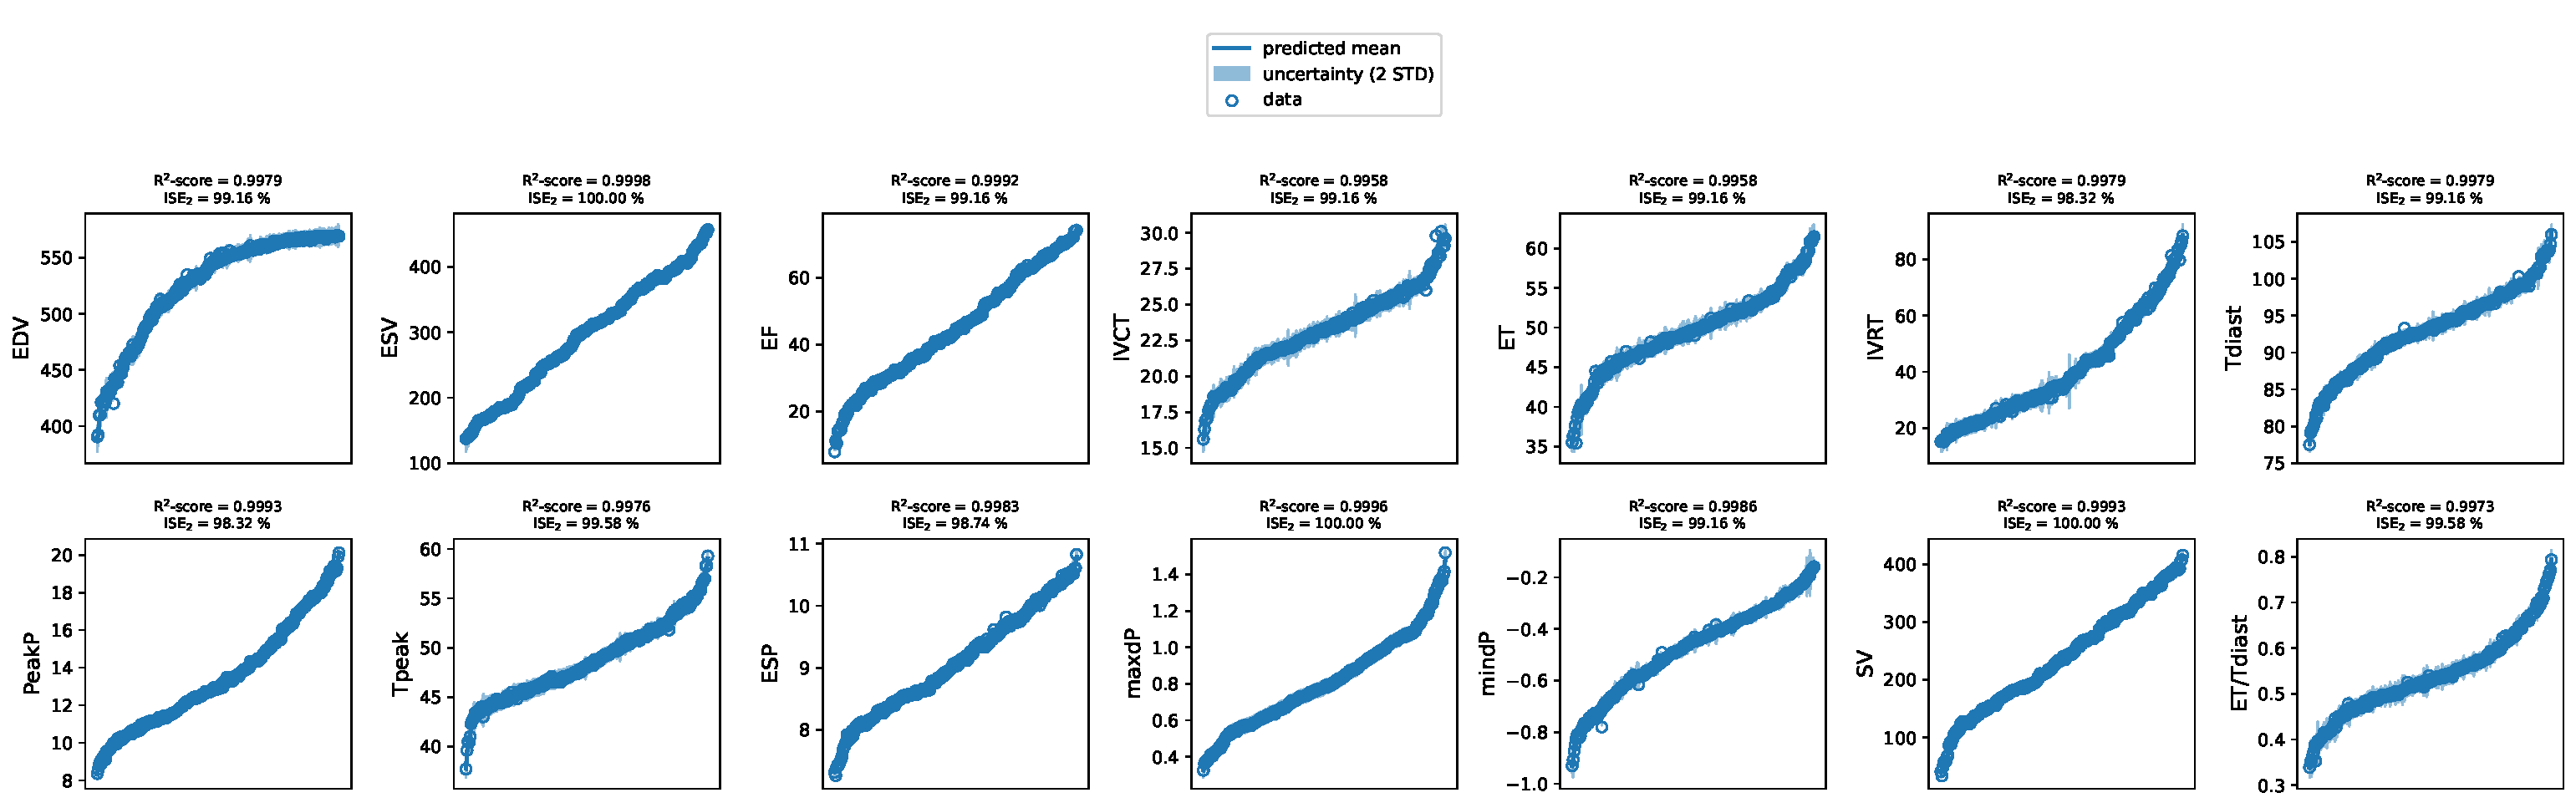
\includegraphics[width=\textwidth]{figures/chapter05/bgpes_vs_bsplit_om.pdf}
    \caption{For each LV feature, the GPE with the highest $R^2$ split test score is used to make predictions at the respective left-out subset of test points. Predictions are sorted in ascending order for the sake of a better visualisation and joined with a thick blue line, and the respective observations (empty dots) are sorted accordingly. $2$ STD confidence intervals (shaded regions) are also plotted around predicted mean lines.}
    \label{fig:omgpes}
\end{figure}

\vspace{0.2cm}
The performed GSA (Figure~\ref{fig:omgsa}) showed that $\trpnf$ was the most important parameter into explaining the LV features' total variance in the model. The second most important parameter was $\nxb$, followed by $\tref$ and $\kxb$ parameters. It is worth noticing that the two cross-bridge formation-regulating parameters that affect the LV function the most are also the ones that regulate the force-calcium relationship in the rat model.

\begin{figure}[!ht]
    \myfloatalign
    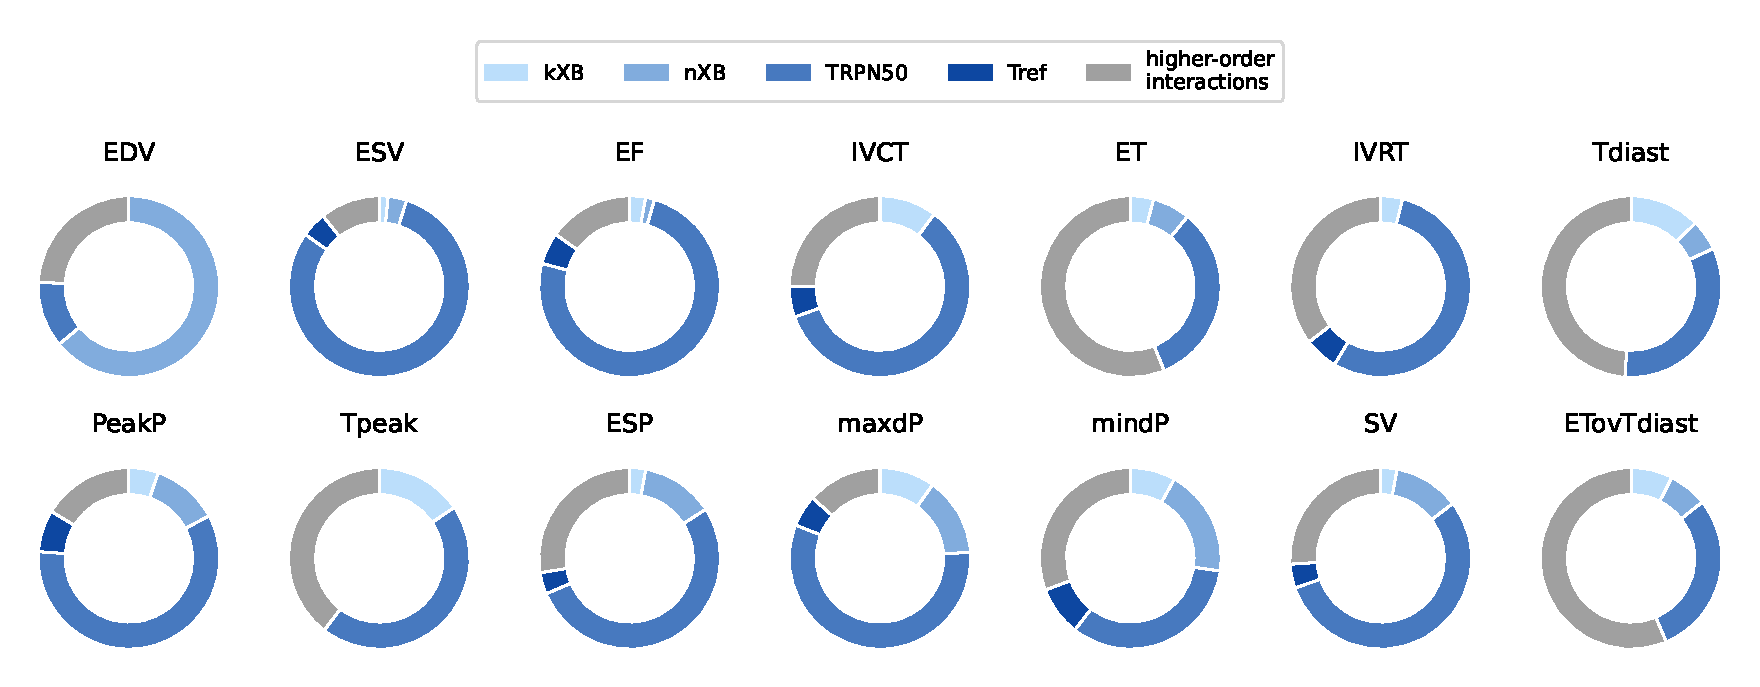
\includegraphics[width=\textwidth]{figures/chapter05/gsa_om.pdf}
    \caption{The impact of cross-bridge related sarcomere parameters on organ-scale LV features in the healthy rat. The contribution of each parameter is represented by its Sobol' main effect. For each LV feature, higher-order interactions (coloured in grey) are represented by the sum of all total effects minus the sum of all main effects.}
    \label{fig:omgsa}
\end{figure}



%
%
%
\subsection{Model predicted OM effects on the LV function}
The OM-compatible $2$D sarcomere parameter space inferred from \textit{in vitro} rat F-pCa data is shown in Figure~\ref{fig:deltas}.

\begin{figure}[!ht]
    \myfloatalign
    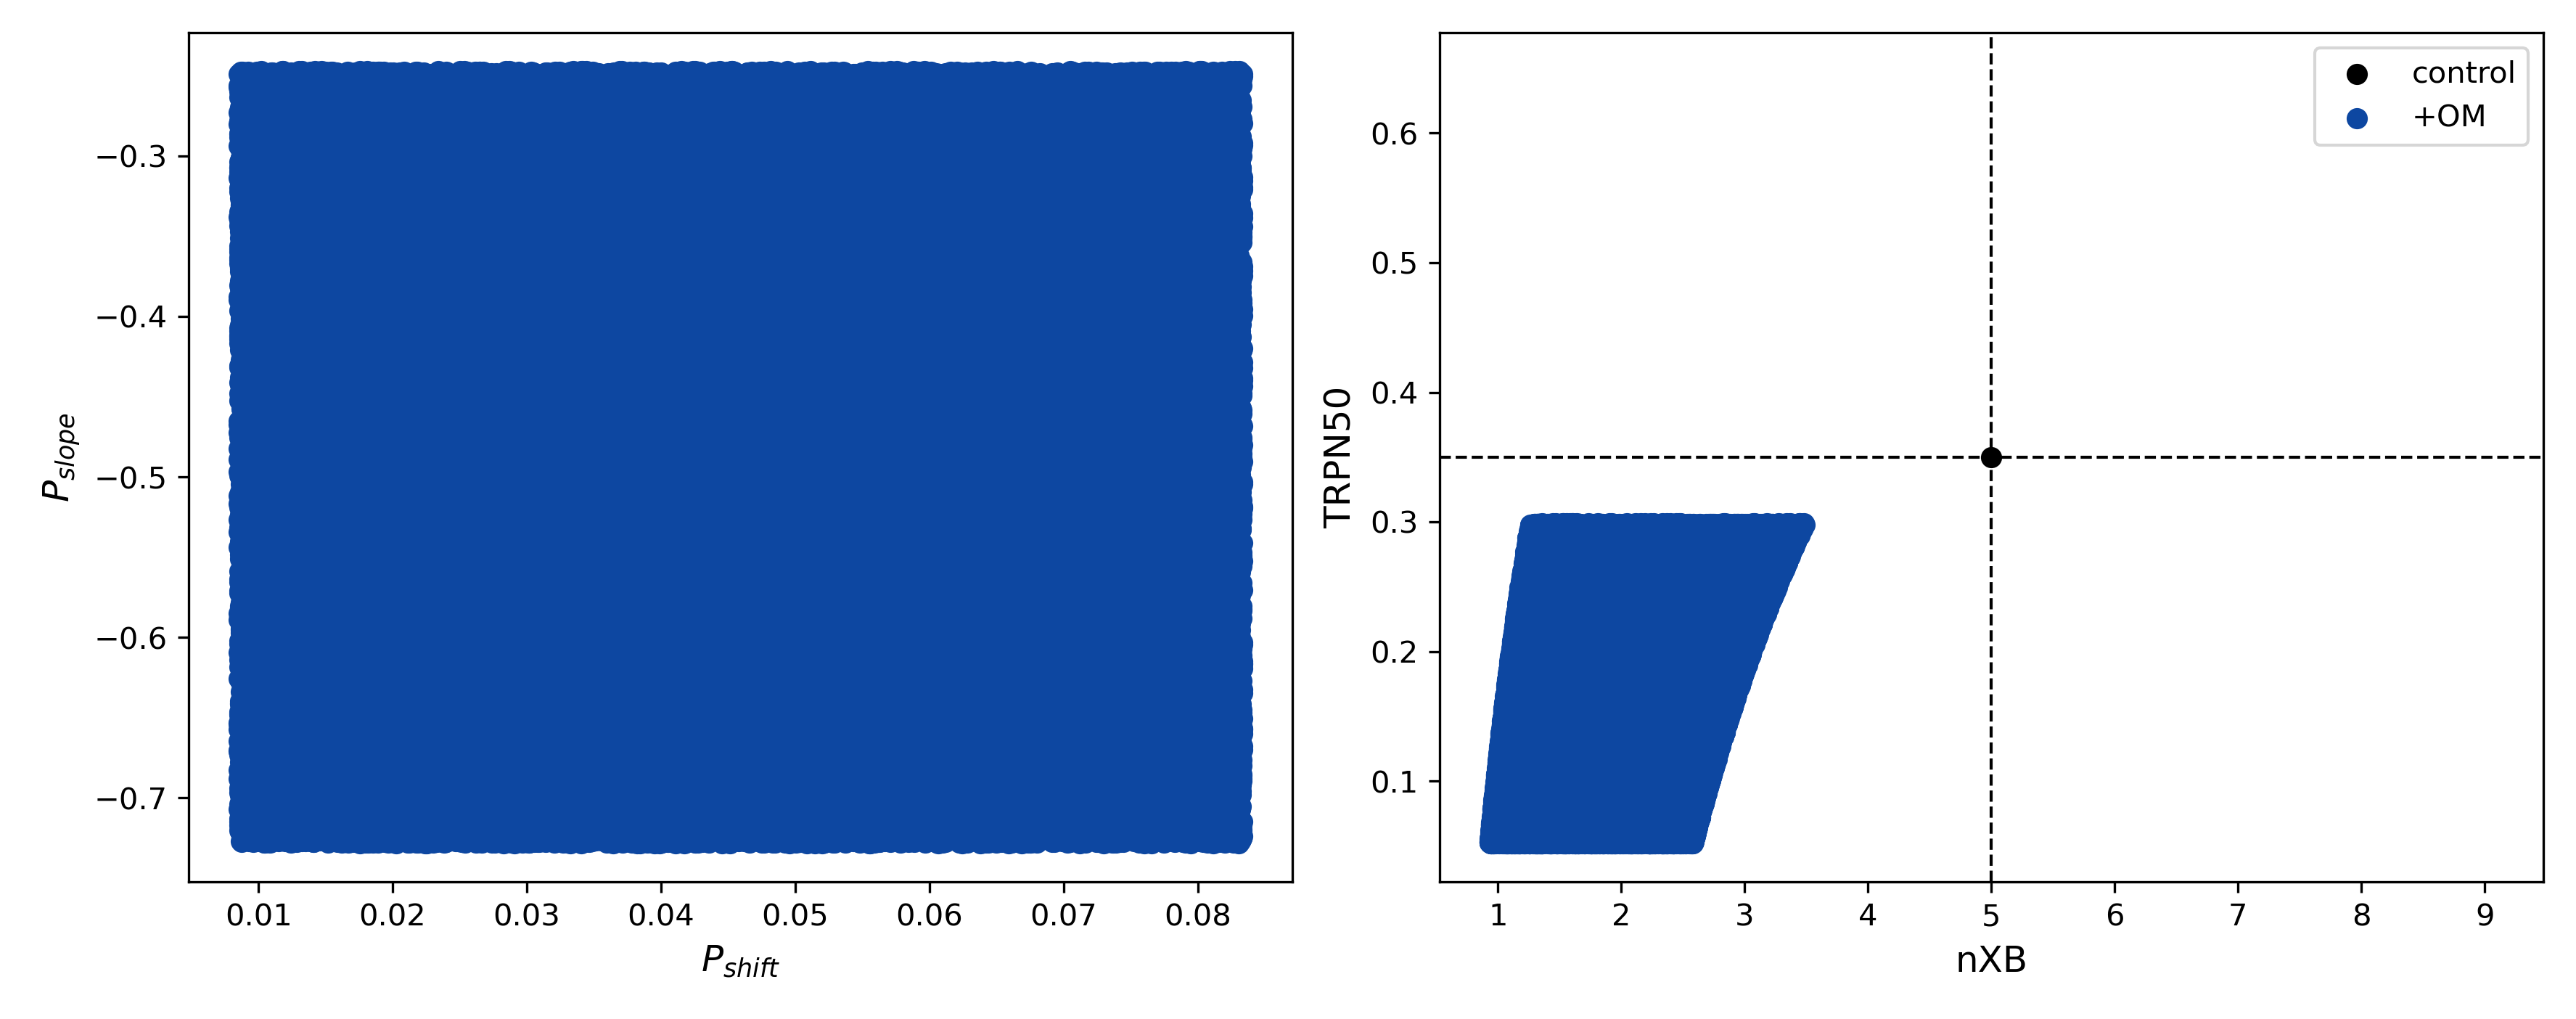
\includegraphics[width=\textwidth]{figures/chapter05/Deltas_and_params_with_OM_blue.png}
    \caption{OM-compatible sarcomere space encoded by the $\nxb$ and $\trpnf$ parameters, inferred from \textit{in vitro} rat F-pCa data. A LHD of $100,000$ points in the ranges of experimental variability of the F-pCa curve (left panel) is projected into the corrisponding plausible $2$D sarcomere parameter space (right panel). The reference parameter set is represented by a black dot, while reference dashed black lines divide the plane in four parts to highlight the quadrant of OM action.}
    \label{fig:deltas}
\end{figure}

\vspace{0.2cm}
Figure~\ref{fig:lvfeatsdistr} shows that the corresponding inferred median effects of these changes to $\pCaf$ and $h$ due to OM on whole-organ function show a qualitative agreement in the direction of change for all the $4$ LV features reported to be significantly altered by OM in the pig study~\cite{Bakkehaug:2015}.

\begin{figure}[!ht]
    \myfloatalign
    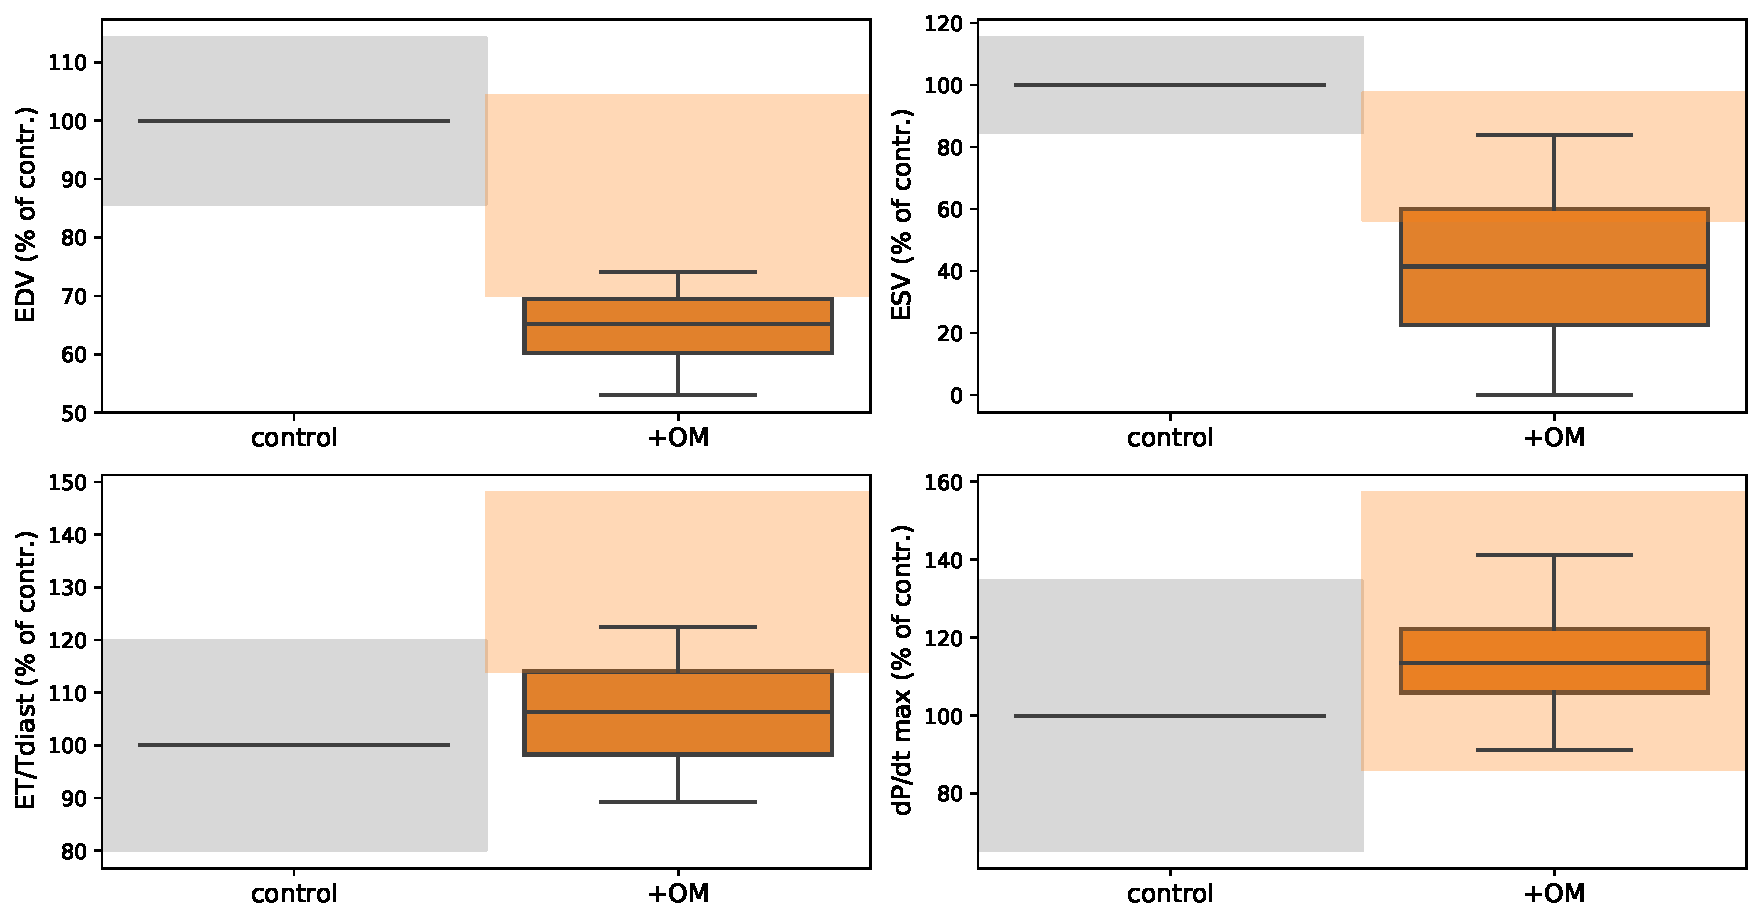
\includegraphics[width=\textwidth]{figures/chapter05/Fig3.pdf}
    \caption{Predicted \textit{in silico} OM effects on whole-heart function as percentage changes of LV features' values from control values. Experimental uncertainty ranges are displayed as shaded regions using percentage-from-control mean $\pm$ standard deviation values for both the healthy (gray) and $+$OM (orange) cases.}
    \label{fig:lvfeatsdistr}
\end{figure}


%
%
%
\subsection{Model predicted OM effects on the F-pCa relationship}\label{sec:ch5inferringomeffectsfpcawholeorganresults}
HM first wave identified $3,469$ points (corresponding to $\SI{0.8672}{\percent}$ of the initial space) as non-implausible for replicating the organ-scale effects of OM administration. The resulting OM-compatible $4$D sarcomere parameter space inferred from \textit{in vivo} pig hemodynamic data is shown in Figure~\ref{fig:wave0}. 

\begin{figure}[!ht]
    \myfloatalign
    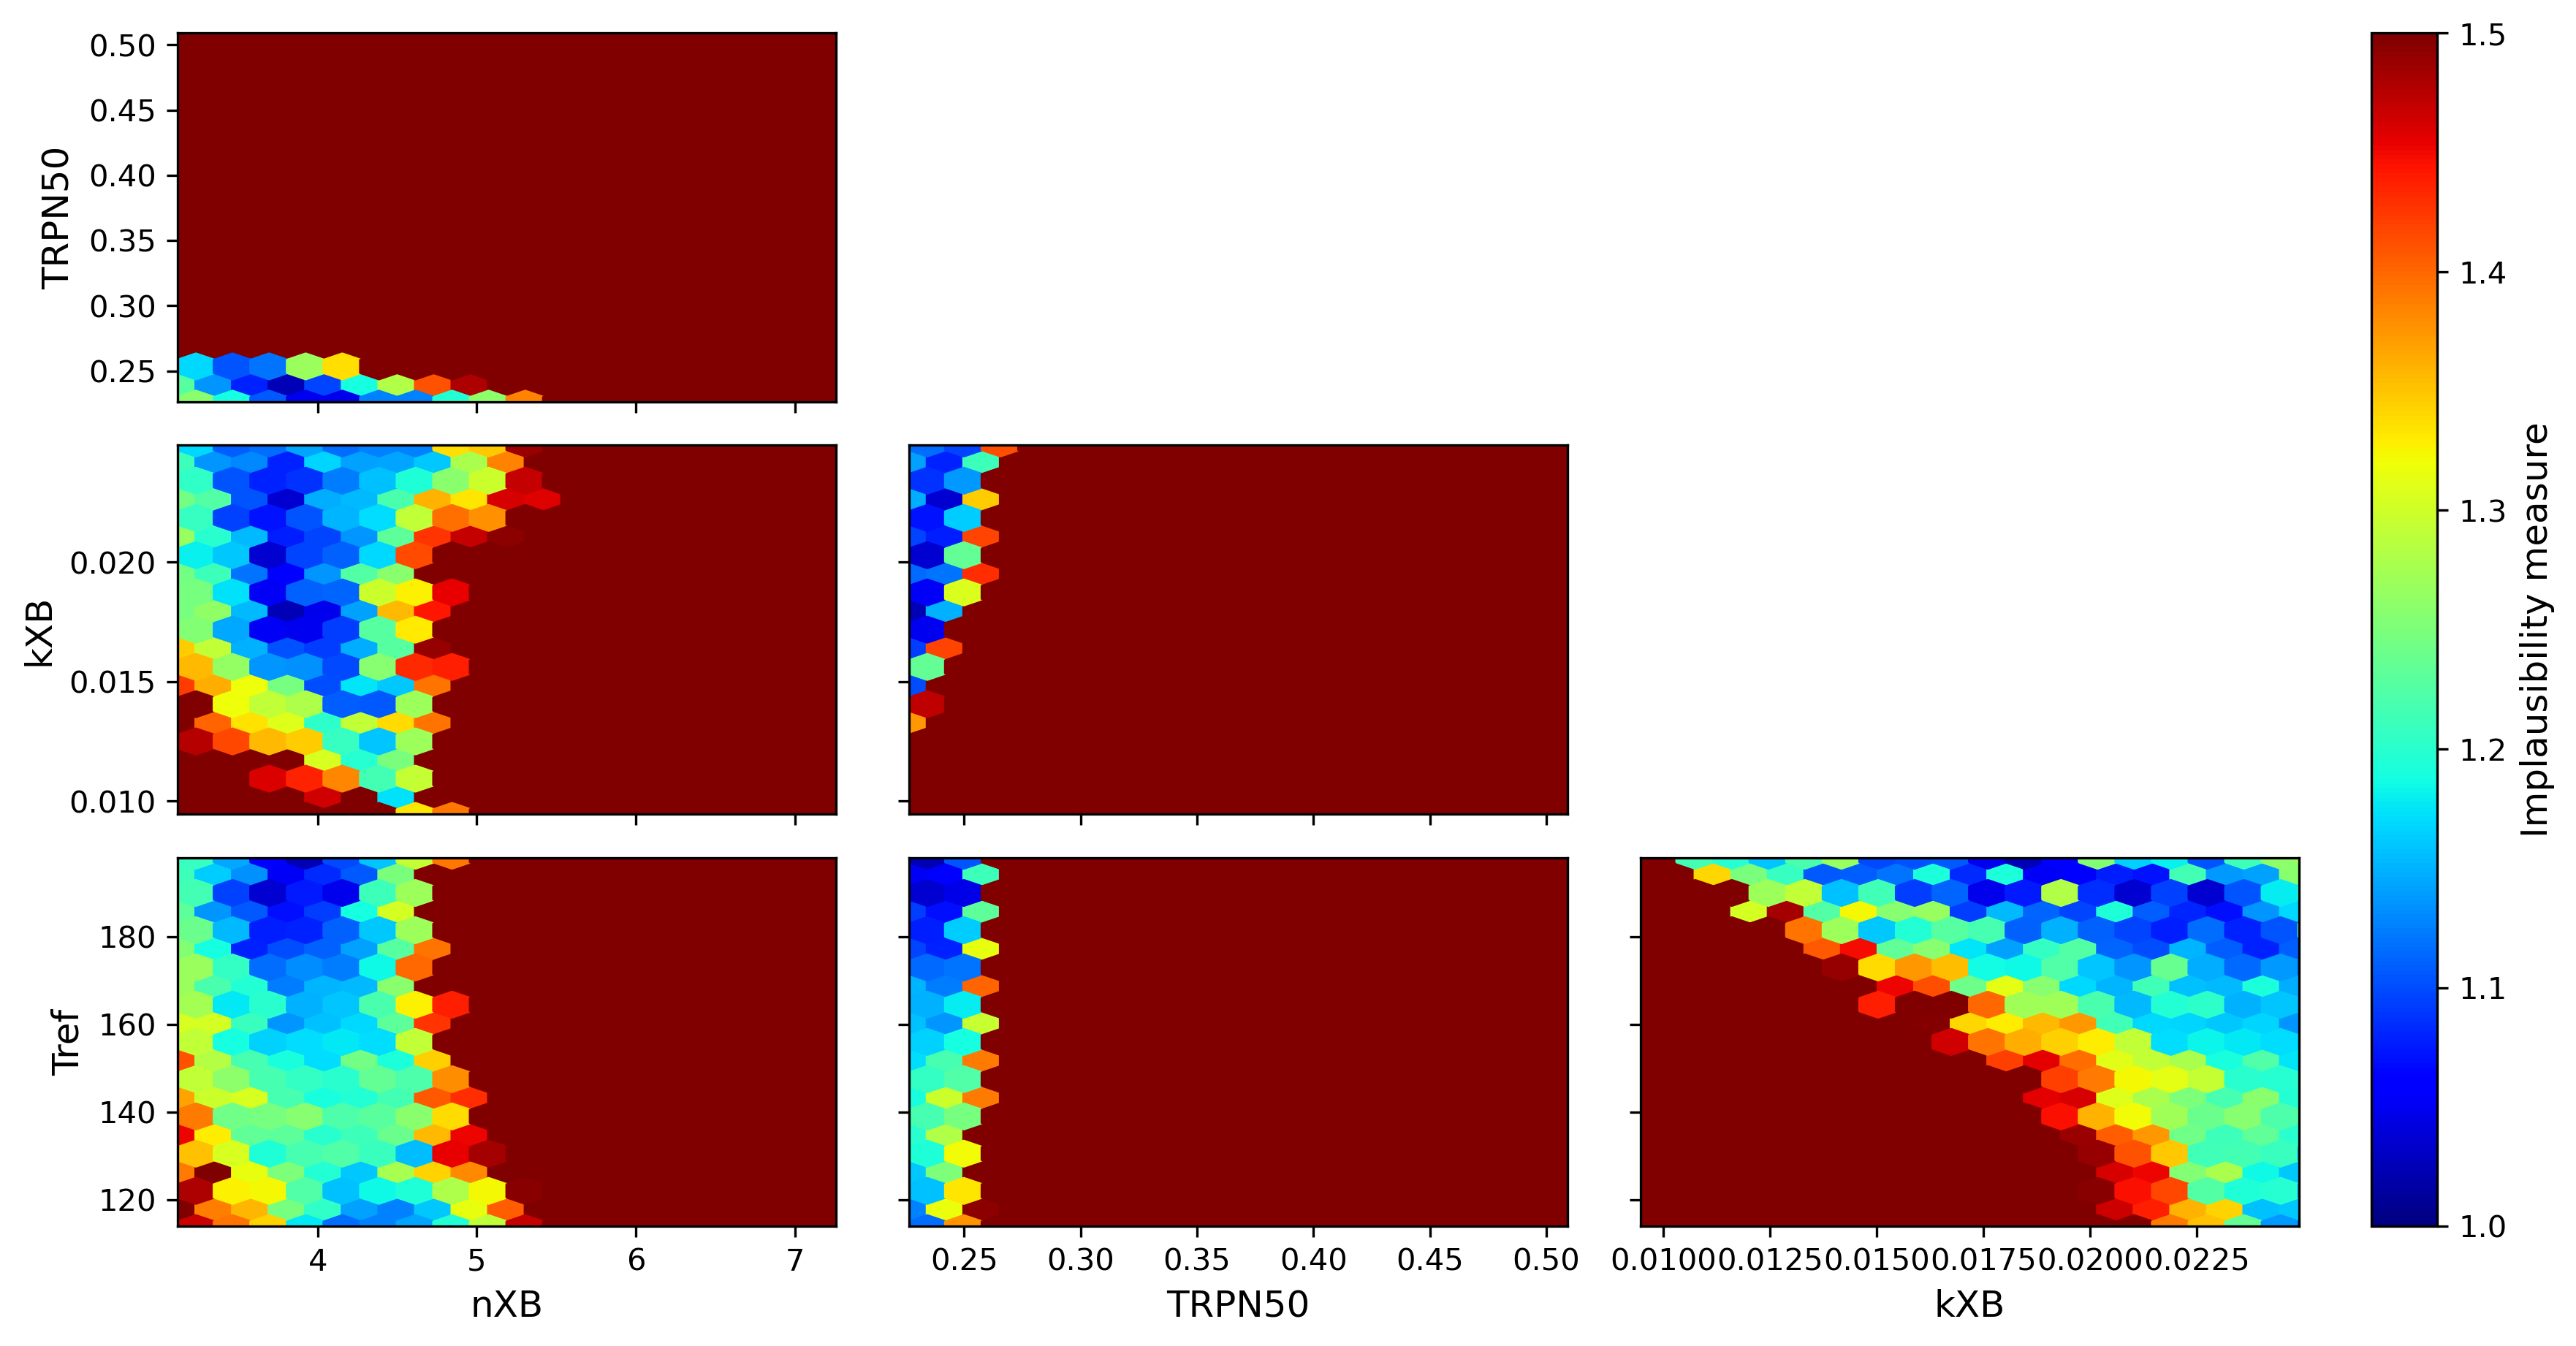
\includegraphics[width=\textwidth]{figures/chapter05/Fig1.png}
    \caption{OM-compatible sarcomere space encoded by the $\kxb$, $\nxb$, $\trpnf$ and $\tref$ parameters, inferred from \textit{in vivo} pig hemodynamic data. This space is obtained by running one iteration of HM which constrains the full parameter space according to an implausibility criterion that evaluates how plausible is a point to yield model predictions that are matching experimental observations.}
    \label{fig:wave0}
\end{figure}

\vspace{0.2cm}
Figure~\ref{fig:wave0mappingtofpCa} shows that the corresponding inferred median effects of these changes to the LV function due to OM on the intact F-pCa curve show a qualitative agreement in the direction of change for both the $\pCaf$ and $h$ features reported to be altered by OM in the rat skinned muscle studies~\cite{Nagy:2015, Kampourakis:2018, Kieu:2019}.

\begin{figure}[!ht]
    \myfloatalign
    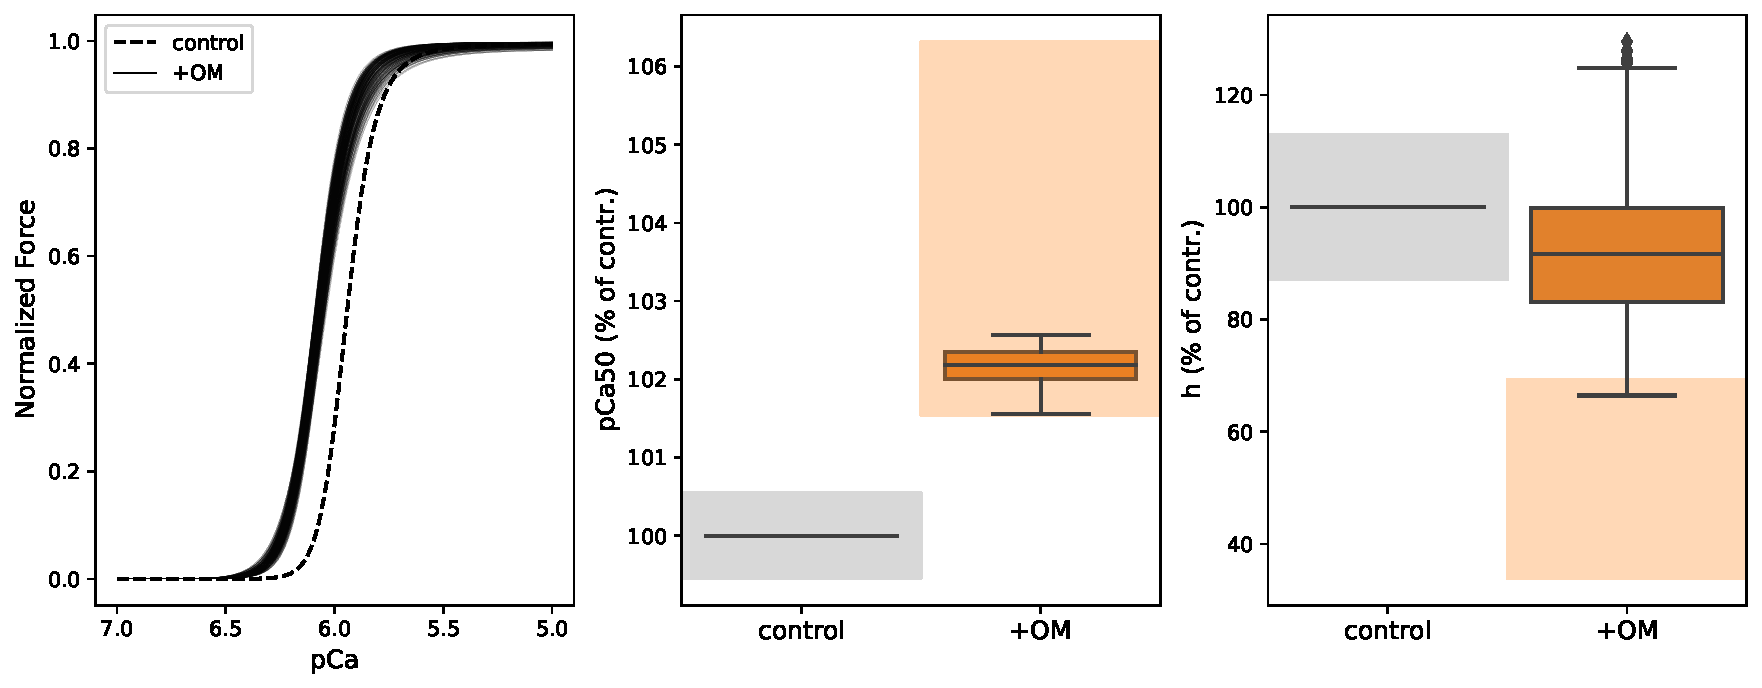
\includegraphics[width=\textwidth]{figures/chapter05/Fig2.pdf}
    \caption{Predicted \textit{in silico} OM effects on the sarcomere as described by F-pCa curves calculated from the constrained, OM-compatible sarcomere parameter space and by the related percentage changes of $\pCaf$ and $h$ values from control values. Experimental uncertainty ranges are displayed (the middle and far right panels) as shaded regions using percentage-from-control mean $\pm$ standard deviation values for both the healthy (gray) and $+$OM (orange) cases.}
    \label{fig:wave0mappingtofpCa}
\end{figure}


%
%
%
\newpage
\section{Discussion}\label{sec:ch5discussion}
\todo{this is Discussion, Limitations, Conclusion copy-pasted from the paper: adapt it to thesis}

\noindent
We have demonstrated that our virtual rat heart framework~\cite{Longobardi:2020} can recapitulate the effects of OM on cardiac contraction and that multi-scale cardiac mechanics models can be used to infer the impact of drugs on cellular function from whole-organ observations. Calibration of model parameters to both cellular and whole-organ data on OM gives us additional insight into the mechanistic processes that link cellular and whole-heart contraction. Our results demonstrate that in order to reproduce available data, OM requires to alter the function of both thick and thin filaments. The OM effect on thick filament (the direct site of action of OM) is essential to reproduce OM effect on tension in whole-heart. Simulations show that the OM effect on F-pCa curves involve changes in thin filament function, namely by altering calcium myofilament sensitivity, which supports the recent hypothesis of the effect OM on thin filaments~\cite{Swenson:2017}.

\vspace{0.2cm}
Limitations of this work include: (1) Both thin and thick filament dynamics are modeled using a simplified representation of the sarcomere, without a detailed mechanistic description of its components. Specifically, the cross-bridge kinetics is described by a two-state model where the strongly-/weakly-/un-bound states are collapsed into a single state. While more detailed models exist~\cite{Land:2015}, their parameters are not necessarily constrained using experimental data due to difficulties in measuring subcellular processes. (2) As a result of (1), the OM effect is modelled using $2$- to $4$-parameters linked to the cross-bridge cycling but not directly incorporating the OM mechanism of action (which is to increase the rate of myosin-head attachment to actin~\cite{Malik:2011}). (3) OM whole-organ data in healthy animals is limited. To the best of our knowledge, the \textit{in vivo} pig hemodynamics data~\cite{Bakkehaug:2015} used to constrain the model parameters is the only available non-human study of OM effect on LV function with therapeutic doses in healthy animals. (4) Differences across species and in acute vs chronic OM administration are not explored. For example, studies in healthy volunteers~\cite{Teerlink:2011} suggest an increase in SV and EF following OM treatment as a result of the overall systolic function improvement. However, we only mapped LV features' values that were reported to significantly change from control after OM administration~\cite{Bakkehaug:2015}, thus our results excluded cases when change in SV and EF features was observed. Additional studies are needed to investigate species differences and chronic effect of OM. (5) We have shown that the median model predictions qualitatively match the observed changes due to OM at the tissue and whole-organ scale. However, the model does not quantitatively match experimental observations. Specifically, there are some non-implausible Hill coefficients in Figure~\ref{fig:wave0mappingtofpCa} that are increased and so do not qualitatively match the experimentally observed changes. Similarly, in some cases $\textrm{ET}/\textrm{Tdiast}$ is predicted to decrease in Figure~\ref{fig:lvfeatsdistr}, in contrast to the experimental observations. There are four potential contributors to this discrepancy. First, the tissue and organ drug effects are taken from different species. Second, the reference model parameters and anatomy are determined from a distinct set of experiments from the OM measurements. Third, the model is a simplification and may be missing some features. Forth, the experiments are performed in skinned preparations, while the model replicates intact tissue. This likely explains the discrepancy in predicted change in Hill coefficient, which is sensitive to the skinning process. Finally, we fitted the model to the data using an emulator, which itself has uncertainty, and this can increase the overall uncertainty. A self-consistent multi-scale data of the effects of OM on cell, tissue and organ scales would allow us to better identify and address the source of these discrepancies.

\vspace{0.2cm}
We demonstrated how multi-scale heart contraction models can aid our understanding of the mechanistic links between cellular and whole-organ function and can help in interpreting skinned experimental preparations in the context of \textit{in vivo} whole-heart function.